\section{Casi d'uso}
    \subsection{Attori dei casi d'uso}
    \subsubsection{Attori primari}
    Gli attori che il gruppo ha ritenuto essere i più adeguati sono:
        \begin{itemize}
            \item \textbf{Utente generico:} utente che può navigare nell'e-commerce e può usufruire di alcune funzionalità, come la visualizzazione e la ricerca dei prodotti, che può aggiungere al proprio carrello, la applicazione di filtri e categorie per la ricerca, e infine di potersi autenticare.\\ Inoltre si divide in:
                \begin{itemize}
                    \item \textbf{Utente non autenticato:} è un utente che ha già un account ma che non ha ancora effettuato il login; può quindi reimpostare la sua password nel caso in cui se la sia dimenticata;
                    \item \textbf{Utente autenticato:} un utente autenticato può a sua volta essere:
                        \begin{itemize}
                            \item \textbf{Cliente autenticato:} cliente che ha effettuato il login, può accedere a tutte le funzionalità riservate ai clienti, come l'aggiunta di prodotti al carrello, l'acquisto, la visualizzazione della lista degli ordini, la possibilità di contattare il venditore, la possibilità di effettuare un reso;
                            \item \textbf{Venditore autenticato:} venditore che ha effettuato il login, può accedere alle funzionalità relative all'amministrazione dei prodotti e delle categorie.
                        \end{itemize}
                        \begin{figure}[!ht]
                            \caption{Attori primari}
                            \vspace{5px}
                            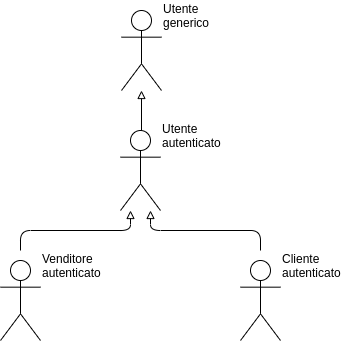
\includegraphics[scale=0.6]{../../../Images/AnalisiRequisiti/attori}
                            \centering
                        \end{figure}
                \end{itemize}
        \end{itemize}
        \subsubsection{Attori secondari}
        \begin{itemize}
            \item \textbf{Servizio di autenticazione esterno:} servizio esterno per il login e per la gestione delle credenziali;
            \item \textbf{Stripe:} servizio esterno per la gestione dei pagamenti.
        \end{itemize}
        \newpage
    \subsection{Elenco dei casi d'uso}
        \textbf{Utilizzo della piattaforma:}
        \vspace{-10px}
        \begin{figure}[!ht]
            \caption{Casi d'uso che interessano gli utenti}
            \vspace{10px}
            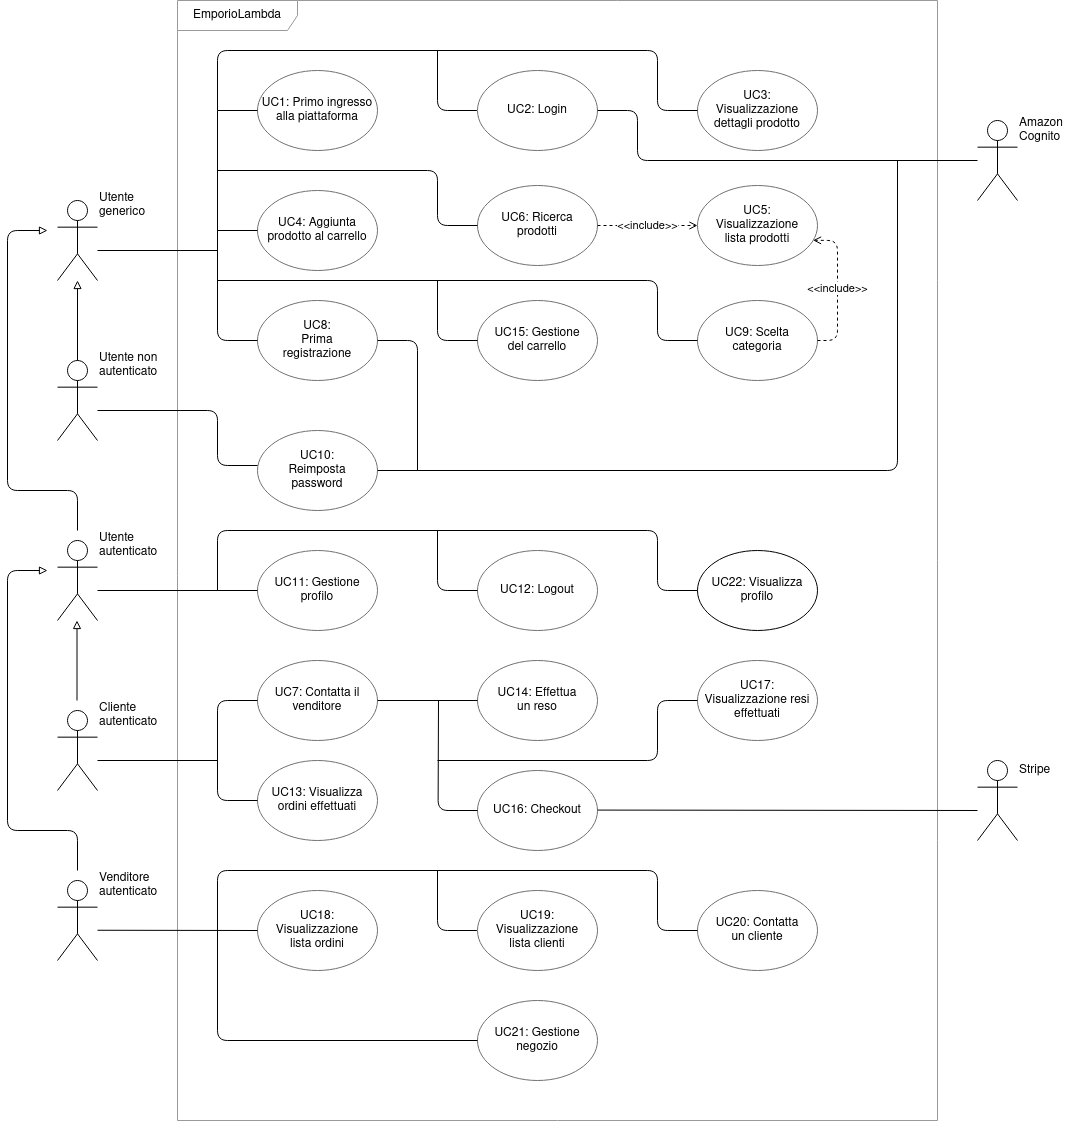
\includegraphics[scale=0.42]{../../../Images/AnalisiRequisiti/casiUso}
            \centering
        \end{figure}
        \newpage
        \subsection{UC1: Autenticazione}
\label{sec:UC1}
\begin{figure}[!ht]
    \caption{Diagramma di UC1: Autenticazione}
    \vspace{10px}
    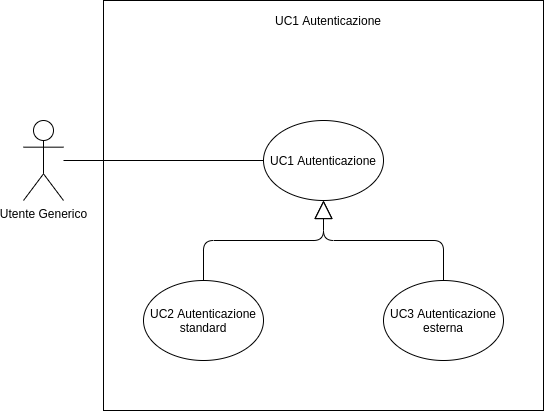
\includegraphics[scale=0.5]{../../../Images/AnalisiRequisiti/UC01}
    \centering
\end{figure}
\begin{itemize}
    \item \textbf{Descrizione:} permette l'autenticazione di un utente;
    \item \textbf{Attore Primario:} utente non autenticato;
    \item \textbf{Attore Secondario:} servizio di autenticazione esterno;
    \item \textbf{Precondizione:} l'utente non si è ancora autenticato
    \item \textbf{Input:} pressione bottone \textit{login};
    \item \textbf{Postcondizione:} l'utente è autenticato;
    \item \textbf{Scenario Principale:}
          \begin{itemize}
              \item l'utente entra nella pagina;
              \item preme il bottone per il login;
              \item viene inderizzato alla pagina di login fornita dal servizio di autenticazione.
          \end{itemize}
\end{itemize}
\newpage
        \subsection{UC2: Autenticazione standard}
\begin{figure}[!ht]
    \caption{Diagramma di UC2: Autenticazione standard}
    \vspace{10px}
    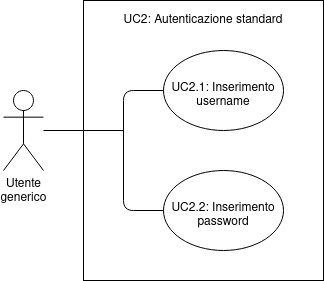
\includegraphics[scale=0.5]{../../../Images/AnalisiRequisiti/UC02}
    \centering
\end{figure}
\label{sec:UC2}
\begin{itemize}
    \item \textbf{Descrizione:} permette l'autenticazione di un utente;
    \item \textbf{Attore Primario:} utente non autenticato;
    \item \textbf{Attore Secondario:} Amazon Cognito;
    \item \textbf{Precondizione:} l'utente è all'interno della pagina di autenticazione;
    \item \textbf{Input:} inserimento dati;
    \item \textbf{Postcondizione:} l'utente è autenticato;
    \item \textbf{Scenario Principale:}
          \begin{itemize}
              \item l'utente è nella pagina dedicata all'autenticazione;
              \item inserisce i propri dati;
              \item preme l'apposito bottone;
              \item l'utente è autenticato.
          \end{itemize}
          \textbf{Estensione:}
          Se lo username o la password non sono corretti:
          \begin{itemize}
              \item viene visualizzato un messaggio di errore (\hyperref[sec:UC33]{\underline{UC33}});
              \item si può ritentare l'inserimento dei dati.
          \end{itemize}
\end{itemize}
\subsubsection{UC2.1: Inserimento username}
\label{sec:UC2.1}
\begin{itemize}
    \item \textbf{Descrizione:} permette l'inserimento del username;
    \item \textbf{Attore Primario:} utente non autenticato;
    \item \textbf{Attore Secondario:} Amazon Cognito;
    \item \textbf{Precondizione:} l'utente è all'interno della pagina di autenticazione;
    \item \textbf{Input:} inserimento username;
    \item \textbf{Postcondizione:} lo username è stato inserito.
\end{itemize}
\subsubsection{UC2.2: Inserimento password}
\label{sec:UC2.2}
\begin{itemize}
    \item \textbf{Descrizione:} permette l'inserimento della password;
    \item \textbf{Attore Primario:} utente non autenticato;
    \item \textbf{Attore Secondario:} Amazon Cognito;
    \item \textbf{Precondizione:} l'utente è all'interno della pagina di autenticazione;
    \item \textbf{Input:} inserimento password;
    \item \textbf{Postcondizione:} la password è stata inserita.
\end{itemize}


        \subsection{UC3: Autenticazione standard}
\begin{figure}[!ht]
    \caption{Diagramma di UC3: Autenticazione standard}
    \vspace{10px}
    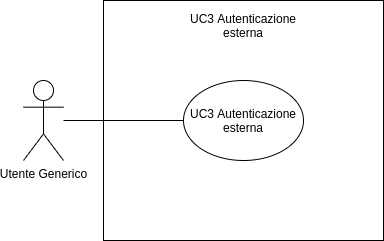
\includegraphics[scale=0.5]{../../../Images/AnalisiRequisiti/UC03}
    \centering
\end{figure}
\label{sec:UC3}
\begin{itemize}
    \item \textbf{Descrizione:} permette l'autenticazione di un utente;
    \item \textbf{Attore Primario:} utente generico;
    \item \textbf{Attore Secondario:} servizio di autenticazione esterno;
    \item \textbf{Precondizione:} l'utente è all'interno della pagina di autenticazione
    \item \textbf{Input:} inserimento dati;
    \item \textbf{Postcondizione:} l'utente è autenticato;
    \item \textbf{Scenario Principale:}
          \begin{itemize}
              \item l'utente è nella pagina dedicata all'autenticazione;
              \item inserisce i propri dati;
              \item preme l'apposito bottone;
              \item l'utente è autenticato.
          \end{itemize}
          \textbf{Estensione:}
          Se la l'username o la password non sono corretti:
          \begin{itemize}
              \item viene visualizzato un messaggio di errore (\hyperref[sec:UC28]{\underline{UC28}});
              \item si può ritentare l'inserimento.
          \end{itemize}
\end{itemize}
\subsubsection{UC3.1: Inseriemtno username}
\label{sec:UC3.1}
\begin{itemize}
    \item \textbf{Descrizione:} permette l'inserimento dell'username;
    \item \textbf{Attore Primario:} utente generico;
    \item \textbf{Attore Secondario:} servizio di autenticazione esterno;
    \item \textbf{Precondizione:} l'utente è all'interno della pagina di autenticazione
    \item \textbf{Input:} inserimento username;
    \item \textbf{Postcondizione:} l'username è stata inserita;
\end{itemize}
\subsubsection{UC3.2: Inseriemtno password}
\label{sec:UC3.2}
\begin{itemize}
    \item \textbf{Descrizione:} permette l'inserimento della password;
    \item \textbf{Attore Primario:} utente generico;
    \item \textbf{Attore Secondario:} servizio di autenticazione esterno;
    \item \textbf{Precondizione:} l'utente è all'interno della pagina di autenticazione
    \item \textbf{Input:} inserimento password;
    \item \textbf{Postcondizione:} la password è stata inserita;
\end{itemize}

        \subsection{UC2: Autenticazione esterna}
        \label{sec:UC2}
        \begin{itemize}
            \item \textbf{Descrizione:} permette l'autenticazione di un utente;
            \item \textbf{Attore Primario:} utente generico;
            \item \textbf{Attore Secondario:} Amazon Cognito;
            \item \textbf{Precondizione:} l'utente generico non si è ancora autenticato
            \item \textbf{Input:} pressione bottone login;
            \item \textbf{Postcondizione:} l'utente è autenticato;
            \item \textbf{Scenario Principale:} 
            \begin{itemize}
                \item l'utente entra nella pagina
                \item preme il bottone per il login
                \item viene inderizzato alla pagina di login fornita da \textit{Amazon Cognito}.
            \end{itemize}
        \end{itemize}
        \subsection{UC5: Visualizzazione dei dettagli di un prodotto}
\label{sec:UC5}
\begin{itemize}
    \item \textbf{Descrizione:} l'utente può visualizzare i dettagli di un prodotto di suo interesse;
    \item \textbf{Attore Primario:} utente generico
    \item \textbf{Precondizione:} l'utente generico si trova nella pagina della lista dei prodotti (\hyperref[sec:UC8]{\underline{UC8}});
    \item \textbf{Input:} click sul prodotto (icona, immagine, nome);
    \item \textbf{Postcondizione:} l'utente visualizza i dettagli del prodotto d'interesse;
    \item \textbf{Scenario Principale:}
          \begin{itemize}
              \item l'utente si trova nella lista dei prodotti;
              \item l'utente visualizza un prodotto di suo interesse;
              \item l'utente lo apre e ne visualizza i dettagli.
          \end{itemize}
\end{itemize}
        \subsection{UC6: Aggiunta di un prodotto al carrello}
        \label{sec:UC6}
        \begin{itemize}
            \item \textbf{Descrizione:} l'utente aggiunge al carrello un prodotto che intende acquistare;
            \item \textbf{Attore Primario:} utente generico;
            \item \textbf{Precondizione:} l'utente generico di trova nella pagina dettagliata del prodotto (\hyperref[sec:UC3]{\underline{UC3}});
            \item \textbf{Input:} click sul bottone di aggiunta al carrello;
            \item \textbf{Postcondizione:} il prodotto è stato aggiunto al carrello;
            \item \textbf{Scenario Principale:}
            \begin{itemize}
                \item l'utente si trova nella pagina dei dettagli del prodotto;
                \item l'utente clicca il bottone per aggiungere il prodotto al carrello;
                \item il prodotto si trova nel carrello.
            \end{itemize}
        \end{itemize}
        
        \subsection{UC7: Ricerca dei prodotti}
        \label{sec:UC7}
        \begin{itemize}
            \item \textbf{Descrizione:} l'utente vuole ricercare un prodotto in base ad una parola chiave; 
            \item \textbf{Attore Primario:} utente generico;
            \item \textbf{Precondizione:} l'utente si trova in una pagina dedicata alla ricerca; 
            \item \textbf{Input:} stringa relativa a ciò che si vuole cercare;
            \item \textbf{Postcondizione:} l'utente visualizza i prodotti corrispondenti alla parola chiave;
            \item \textbf{Scenario Principale:}
            \begin{itemize}
                \item l'utente vuole ricercare un prodotto secondo una determinata parola chiave;
                \item gli vengo mostrati tutti i risultati della ricerca nella lista dei prodotti.
            \end{itemize}
            \item \textbf{Inclusioni:}
            \begin{itemize}
                \item viene visualizzata una pagina con tutti i risultati della ricerca (\hyperref[sec:UC6]{\underline{UC6}}).
            \end{itemize}
        \end{itemize}
        \subsection{UC8: Visualizzazione della lista dei prodotti}
\label{sec:UC8}
\begin{figure}[!ht]
    \caption{Diagramma di UC8: Visualizzazione della lista dei prodotti}
    \vspace{10px}
    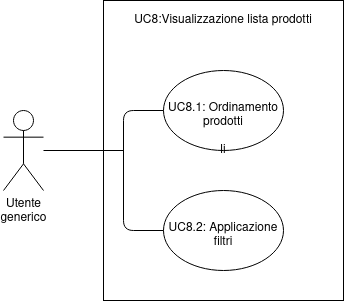
\includegraphics[scale=0.5]{../../../Images/AnalisiRequisiti/UC08.png}
    \centering
\end{figure}
\begin{itemize}
    \item \textbf{Descrizione:} l'utente visualizza la pagina della lista dei prodotti;
    \item \textbf{Attore Primario:} utente generico;
    \item \textbf{Precondizione:} l'utente si trova in una qualsiasi pagina della piattaforma;
    \item \textbf{Postcondizione:} l'utente visualizza la pagina con la lista dei prodotti;
    \item \textbf{Scenario Principale:}
          \begin{itemize}
              \item l'utente è in una pagina della piattaforma;
              \item cerca un prodotto o sceglie una categoria;
              \item l'utente visualizza la lista dei prodotti;
          \end{itemize}
\end{itemize}
\subsubsection{UC8.1: Ordinamento prodotti}
\label{sec:UC8.1}
\begin{itemize}
    \item \textbf{Descrizione:} l'utente seleziona la modalità in cui visualizzare i file;
    \item \textbf{Attore Primario:} utente generico;
    \item \textbf{Precondizione:} l'utente si trova all'interno della pagina con la lista dei prodotti (\hyperref[sec:UC8]{\underline{UC8}});
    \item \textbf{Input:} selezione del parametro scelto;
    \item \textbf{Postcondizione:} la lista dei prodotti si aggiorna secondo l'ordinamento scelto;
    \item \textbf{Scenario Principale:}
          \begin{itemize}
              \item l'utente si trova all'interno della pagina con la lista dei prodotti;
              \item inserisce i parametri per ordinare i prodotti;
              \item la pagina con la lista dei prodotti si aggiorna con i prodotti ordinati.
          \end{itemize}
\end{itemize}
\subsubsection{UC8.2: Applicazione filtri}
\label{sec:UC8.2}
\begin{itemize}
    \item \textbf{Descrizione:} l'utente filtra i prodotti in base alle loro caratteristiche;
    \item \textbf{Attore Primarilo:} utente generico
    \item \textbf{Precondizione:} l'utente si trova all'interno della pagina con la lista dei prodotti (\hyperref[sec:UC8]{\underline{UC8}});
    \item \textbf{Input:} selezione del filtro desiderato;
    \item \textbf{Postcondizione:} la pagina si aggiorna secondo i filtri selezionati;
    \item \textbf{Scenario Principale:}
          \begin{itemize}
              \item l'utente si trova all'interno della pagina con la lista dei prodotti;
              \item inserisce i parametri per filtrare i prodotti;
              \item la pagina con la lista dei prodotti si aggiorna con i prodotti filtrati.
          \end{itemize}
\end{itemize}
        \subsection{UC9: Registrazione}
\label{sec:UC9}
\begin{itemize}
    \item \textbf{Descrizione:} l'utente non si è mai registrato nella piattaforma;
    \item \textbf{Attore Primario:} utente generico;
    \item \textbf{Attore Secondario:} Amazon Cognito;
    \item \textbf{Precondizione:} l'utente non ha un profilo nella piattaforma;
    \item \textbf{Input:} pressione apposito bottone;
    \item \textbf{Postcondizione:} l'utente viene reinderizzato alla pagina Amazon cognito per la registrazione;
    \item \textbf{Scenario Principale:}
    \begin{itemize}
        \item un utente arriva per la prima volta nella piattaforma;
        \item si registra attraverso la piattaforma Amazon Cognito dove potrà registrarsi inserendo:
        \begin{itemize}
            \item nome;
            \item cognome;
            \item username;
            \item password;
            \item ripetizione password.
        \end{itemize}
    \end{itemize} 
\end{itemize}
        \subsection{UC10: Registrazione esterna}
\label{sec:UC10}
\begin{itemize}
    \item \textbf{Descrizione:} l'utente non si è mai registrato nella piattaforma;
    \item \textbf{Attore Primario:} utente non autenticato;
    \item \textbf{Attore Secondario:} servizio di autenticazione esterno;
    \item \textbf{Precondizione:} l'utente non ha un profilo nella piattaforma;
    \item \textbf{Input:} pressione apposito bottone;
    \item \textbf{Postcondizione:} l'utente viene indirizzato alla pagina del servizio di autenticazione esterno per la registrazione;
    \item \textbf{Scenario Principale:}
          \begin{itemize}
              \item un utente arriva per la prima volta nella piattaforma;
              \item si registra attraverso il servizio di autenticazione esterno dove dovrà inserire:
                    \begin{itemize}
                        \item nome;
                        \item cognome;
                        \item username;
                        \item password;
                        \item ripetizione password.
                    \end{itemize}
          \end{itemize}
\end{itemize}
        \subsection{UC11: Registrazione esterna}
\label{sec:UC11}
\begin{itemize}
    \item \textbf{Descrizione:} l'utente non si è mai registrato nella piattaforma;
    \item \textbf{Attore Primario:} utente generico;
    \item \textbf{Attore Secondario:} servizio di autenticazione esterno;
    \item \textbf{Precondizione:} l'utente non ha un profilo nella piattaforma;
    \item \textbf{Input:} pressione apposito bottone;
    \item \textbf{Postcondizione:} l'utente viene reinderizzato alla pagina del servizio di autenticazione esterno per la registrazione;
    \item \textbf{Scenario Principale:}
          \begin{itemize}
              \item un utente arriva per la prima volta nella piattaforma;
              \item si registra attraverso il servizio di autenticazione esterno dove potrà registrarsi inserendo:
                    \begin{itemize}
                        \item nome;
                        \item cognome;
                        \item username;
                        \item password;
                        \item ripetizione password.
                    \end{itemize}
          \end{itemize}
\end{itemize}
        
\subsection{UC12: Rimozione di un prodotto dal carrello}
\label{sec:UC12}
\begin{itemize}
    \item \textbf{Descrizione:} sezione per rimuovere un prodotto dal carrello;
    \item \textbf{Attore Primario:} utente non autenticato, utente autenticato;
    \item \textbf{Precondizione:} l'utente è nella pagina del carrello (\hyperref[sec:UC11]{\underline{UC11}});
    \item \textbf{Input:} l'utente seleziona il prodotto da rimuovere dal carrello;
    \item \textbf{Postcondizione:} viene rimosso il prodotto selezionato.
\end{itemize}
        
\subsection{UC13: Modifica della quantità di un prodotto nel carrello}
\label{sec:UC13}
\begin{itemize}
    \item \textbf{Descrizione:} sezione per modificare la quantità di un prodotto nel carrello;
    \item \textbf{Attore Primario:} utente non autenticato;
    \item \textbf{Precondizione:} l'utente è nella pagina del carrello (\hyperref[sec:UC11]{\underline{UC11}});
    \item \textbf{Input:} l'utente seleziona la nuova quantità desiderata per il prodotto;
    \item \textbf{Postcondizione:} le modifiche sono applicate;
    \item \textbf{Estensioni:}
          \begin{itemize}
              \item se la quantità inserita dovesse superare la quantità disponibile, l'utente viene avvisato (\hyperref[sec:UC14]{\underline{UC14}}).
          \end{itemize}
\end{itemize}
        \subsection{UC14: Reimposta password}
\label{sec:UC14}
\begin{itemize}
    \item \textbf{Descrizione:} l'utente non ricorda le prorpie credenziali;
    \item \textbf{Attore Primario:} utente generico;
    \item \textbf{Attore Secondario:} servizio di autenticazione esterno;
    \item \textbf{Precondizione:} l'utente si trova nella pagina di login;
    \item \textbf{Input:} pressione apposito bottone;
    \item \textbf{Postcondizione:} l'utente viene reindirizzato alla pagina di recupero password;
    \item \textbf{Scenario Principale:}
          \begin{itemize}
              \item un utente non ancora autenticato, non ricorda la proprio password;
              \item procede con la procedura di recupero.
          \end{itemize}
\end{itemize}
        \subsection{UC15: Scelta della categoria}
\label{sec:UC15}
\begin{itemize}
    \item \textbf{Descrizione:} l'utente sceglie una specifica categoria di prodotti da ricercare;
    \item \textbf{Attore Primario:} utente non autenticato;
    \item \textbf{Precondizione:} l'utente si trova in una pagina che consente la divisione in categorie;
    \item \textbf{Input:} selezione della categoria;
    \item \textbf{Postcondizione:} la categoria di ricerca cambia secondo la scelta dell'utente;
    \item \textbf{Scenario Principale:}
          \begin{itemize}
              \item l'utente vuole ricercare un prodotto appartenente ad una determinata categoria.
          \end{itemize}
    \item \textbf{Inclusioni:}
          \begin{itemize}
              \item viene visualizzata una pagina con tutti i risultati della ricerca (\hyperref[sec:UC7]{\underline{UC7}}).
          \end{itemize}
\end{itemize}
        \subsection{UC16: Visualizzazione profilo}
\label{sec:UC16}
\begin{itemize}
    \item \textbf{Descrizione:} l'utente vuole visualizzare le informazioni del proprio profilo;
    \item \textbf{Attore Primario:} utente autenticato;
    \item \textbf{Attore Secondario:} servizio di autenticazione esterno;
    \item \textbf{Precondizione:} l'utente di trova all'interno della piattaforma;
    \item \textbf{Input:} pressione dell'apposito bottone;
    \item \textbf{Postcondizione:} l'utente viene reindirizzato alla pagina del suo profilo.
    \item \textbf{Scenario Principale:} l'utente entra nel proprio profilo e visualizza le proprie informazioni:
          \begin{itemize}
              \item nome;
              \item cognome;
              \item e-mail;
              \item indirizzi.
          \end{itemize}
\end{itemize}
        \subsection{UC17: Gestione profilo}
\label{sec:UC17}
\begin{figure}[!ht]
    \caption{Diagramma di UC17: Gestione profilo}
    \vspace{10px}
    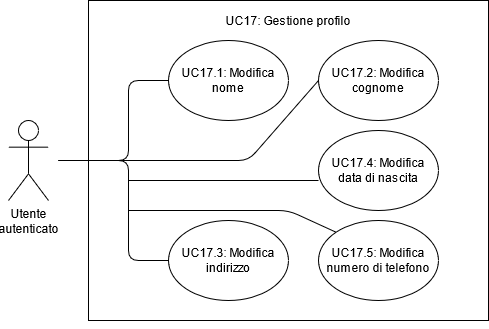
\includegraphics[scale=0.5]{../../../Images/AnalisiRequisiti/UC17}
    \centering
\end{figure}

\begin{itemize}
    \item \textbf{Descrizione:} l'utente vuole gestire il proprio profilo;
    \item \textbf{Attore Primario:} utente autenticato;
    \item \textbf{Attore Secondario:} servizio di autenticazione esterno;
    \item \textbf{Precondizione:} l'utente si trova all'interno del proprio profilo
    \item \textbf{Postcondizione:} l'utente può modificare il proprio profilo
    \item \textbf{Scenario Principale:}
          \begin{itemize}
              \item  l'utente decide cosa modificare tra:
                    \begin{itemize}
                        \item nome;
                        \item cognome;
                        \item username;
                        \item password;
                        \item indirizzo.
                    \end{itemize}
          \end{itemize}
\end{itemize}



\subsubsection{UC17.1 Modifica del nome}
\label{sec:UC17.1}
\begin{itemize}
    \item \textbf{Descrizione:} l'utente vuole modificare il proprio nome relativo all'account;
    \item \textbf{Attore Primario:} utente autenticato;
    \item \textbf{Attore Secondario:} servizio di autenticazione esterno;
    \item \textbf{Precondizione:} l'utente si trova all'interno del proprio profilo
    \item \textbf{Postcondizione:} l'utente può modificare il proprio nome.
\end{itemize}

\subsubsection{UC17.2 Modifica del cognome}
\label{sec:UC17.2}
\begin{itemize}
    \item \textbf{Descrizione:} l'utente vuole modificare il proprio cognome relativo all'account;
    \item \textbf{Attore Primario:} utente autenticato;
    \item \textbf{Attore Secondario:} servizio di autenticazione esterno;
    \item \textbf{Precondizione:} l'utente si trova all'interno del proprio profilo
    \item \textbf{Postcondizione:} l'utente può modificare il proprio cognome.
\end{itemize}

\subsubsection{UC17.3 Modifica dell'username}
\label{sec:UC17.3}
\begin{itemize}
    \item \textbf{Descrizione:} l'utente vuole modificare il proprio username;
    \item \textbf{Attore Primario:} utente autenticato;
    \item \textbf{Attore Secondario:} servizio di autenticazione esterno;
    \item \textbf{Precondizione:} l'utente si trova all'interno del proprio profilo;
    \item \textbf{Postcondizione:} l'utente può modificare il proprio username;
    \item \textbf{Estensione}: visualizzazione errore se l'username è già presente nel database \hyperref[sec:UC17.6]{UC17.6}.
\end{itemize}

\subsubsection{UC17.4 Modifica della password}
\label{sec:UC17.4}
\begin{itemize}
    \item \textbf{Descrizione:} l'utente vuole modificare la propria password;
    \item \textbf{Attore Primario:} utente autenticato;
    \item \textbf{Attore Secondario:} servizio di autenticazione esterno;
    \item \textbf{Precondizione:} l'utente si trova all'interno del proprio profilo
    \item \textbf{Postcondizione:} l'utente può modificare la propria password.
\end{itemize}

\subsubsection{UC17.5 Modifica dell'indirizzo}
\label{sec:UC17.5}
\begin{itemize}
    \item \textbf{Descrizione:} l'utente vuole modificare il proprio indirizzo;
    \item \textbf{Attore Primario:} utente autenticato;
    \item \textbf{Attore Secondario:} servizio di autenticazione esterno;
    \item \textbf{Precondizione:} l'utente si trova all'interno del proprio profilo
    \item \textbf{Postcondizione:} l'utente può modificare il proprio indirizzo.
\end{itemize}

\subsubsection{UC17.6: Visualizzazione username già presente}
\label{sec:UC17.6}
\begin{itemize}
    \item \textbf{Descrizione:} Visualizzazione di un errore se lo username è già in uso;
    \item \textbf{Attore Primario:} utente autenticato;
    \item \textbf{Attore Secondario:} servizio di autenticazione esterno;
    \item \textbf{Precondizione:} l'utente ha inserito uno username non disponibile perchè già usato;
    \item \textbf{Postcondizione:} l'utente visualizza un messaggio di errore.
\end{itemize}

\subsubsection{UC17.7: Password non conforme}
\label{sec:UC17.7}
\begin{itemize}
    \item \textbf{Descrizione:} Visualizzazione di un errore se la password non è conforme ai requisiti;
    \item \textbf{Attore Primario:} utente autenticato;
    \item \textbf{Attore Secondario:} Amazon Cognito;
    \item \textbf{Precondizione:} l'utente ha inserito una password non conforme ai requisiti, che sono:
          \begin{itemize}
              \item lunghezza almeno di 8 caratteri;
              \item contenga almeno una lettera maiuscola;
              \item contenga almeno una lettera minuscola;
              \item contenga almeno un numero
              \item contenga almeno un carattere speciale;
          \end{itemize}
    \item \textbf{Postcondizione:} l'utente visualizza un messaggio di errore.
\end{itemize}
        \subsection{UC18: Contatta il venditore}
\label{sec:UC18}
\begin{itemize}
    \item \textbf{Descrizione:} l'utente vuole contattare il venditore;
    \item \textbf{Attore Primario:} utente autenticato
    \item \textbf{Precondizione:} l'utente si trova in una pagina che permette di contattare il venditore;
    \item \textbf{Input:} pressione dell'apposito bottone;
    \item \textbf{Postcondizione:} l'utente può contattare il venditore;
    \item \textbf{Scenario Principale:}
    \begin{itemize}
        \item l'utente contatta il venditore tramite questa sezione.
    \end{itemize}
\end{itemize}
        \subsection{UC19: Checkout}
\label{sec:UC19}
\begin{figure}[!ht]
    \caption{Diagramma di UC19: Checkout}
    \vspace{10px}
    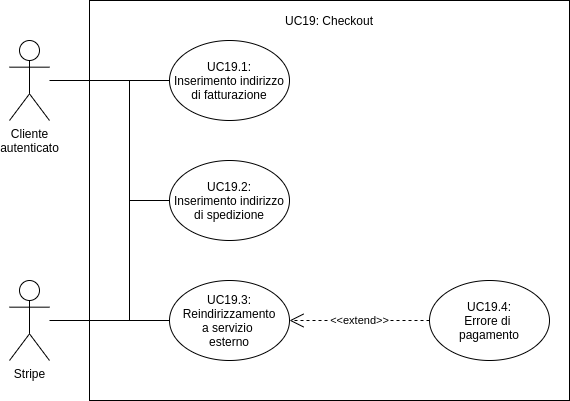
\includegraphics[scale=0.5]{../../../Images/AnalisiRequisiti/UC19}
    \centering
\end{figure}
\begin{itemize}
    \item \textbf{Descrizione:} caso d'uso per la creazione di un nuovo ordine e l'acquisto dei prodotti;
    \item \textbf{Attore Primario:} cliente autenticato;
    \item \textbf{Attore Secondario:} Stripe\textsubscript{\textbf{G}}, gestore di pagamenti di terze parti;
    \item \textbf{Precondizione:} il cliente si trova, nel carrello (\hyperref[sec:UC12]{\underline{UC12}}) e ha già inserito almeno un prodotto oppure nella pagina del prodotto (\hyperref[sec:UC5]{\underline{UC5}});
    \item \textbf{Input:} il cliente clicca il bottone per iniziare il checkout;
    \item \textbf{Postcondizione:} l'ordine viene emesso e aggiunto alla lista degli ordini di quel cliente; i prodotti acquistati vengono rimossi dal carrello e viene diminuita la quantità dal deposito del venditore; il cliente viene reindirizzato alla pagina del riepilogo dell'ordine (\hyperref[sec:UC21]{\underline{UC21}})
    \item \textbf{Scenario Principale:}
          \begin{itemize}
              \item il cliente preme sul pulsante per entrare nella sezione del checkout;
              \item il cliente inserisce i dati di fatturazione (\hyperref[sec:UC19.1]{\underline{UC19.1}}) e, se diversi, i dati di spedizione (\hyperref[sec:UC19.2]{\underline{UC19.2}});
              \item vengono inseriti eventuali costi di spedizione;
              \item il cliente viene reindirizzato al servizio di pagamento esterno, dove inserisce i dati di pagamento;
              \item l'ordine è emesso e segnato come completato.
          \end{itemize}
    \item \textbf{Estensioni:}
    \item Il cliente decide di non completare il checkout:
          \begin{itemize}
              \item  il cliente esce dalla pagina senza causare modifiche al carrello;
          \end{itemize}
\end{itemize}
\subsubsection{UC19.1: Inserimento dell'indirizzo di fatturazione}
\label{sec:UC19.1}
\begin{itemize}
    \item \textbf{Descrizione:} Sezione per l'inserimento dell'indirizzo fatturazione;
    \item \textbf{Attore Primario:} cliente autenticato;
    \item \textbf{Precondizione:} il cliente si trova nella fase di checkout;
    \item \textbf{Input:} il cliente inserisce i dati richiesti dalla pagina;
    \item \textbf{Postcondizione:} si procede con la fase successiva del checkout (\hyperref[sec:UC19.2]{\underline{UC19.2}})
    \item \textbf{Scenario Principale:} il cliente inserisce negli appositi spazi i dati per completare l'indirizzo di fatturazione.
\end{itemize}
\subsubsection{UC19.2: Inserimento dell'indirizzo di spedizione}
\label{sec:UC19.2}
\begin{itemize}
    \item \textbf{Descrizione:} Sezione per l'inserimento dell'indirizzo spedizione;
    \item \textbf{Attore Primario:} cliente autenticato;
    \item \textbf{Precondizione:} il cliente si trova nella fase di checkout;
    \item \textbf{Input:} il cliente inserisce i dati richiesti dalla pagina, oppure clicca un pulsante se l'indirizzo di spedizione è lo stesso di quello di fatturazione;
    \item \textbf{Postcondizione:} si procede con la fase successiva del checkout (\hyperref[sec:UC19.3]{\underline{UC19.3}})
    \item \textbf{Scenario Principale:} il cliente inserisce negli appositi spazi i dati per completare l'indirizzo di spedizione oppure clicca il pulsante per autocompletarli se è il medesimo di quello di fatturazione.
\end{itemize}
\subsubsection{UC19.3: Reindirizzamento al servizio di pagamento esterno}
\label{sec:UC19.3}
\begin{itemize}
    \item \textbf{Descrizione:} Sezione per il pagamento dell'ordine da effettuare;
    \item \textbf{Attore Primario:} cliente autenticato;
    \item \textbf{Attore Secondario:} Stripe, gestore di pagamenti di terze parti;
    \item \textbf{Precondizione:} il cliente ha inserito i dati per la fatturazione e la spedizione nella sezione del checkout;
    \item \textbf{Input:} il cliente preme il pulsante per il pagamento;
    \item \textbf{Postcondizione:} il pagamento ha avuto esito positivo, l'ordine viene confermato e viene decrementata la quantità dei prodotti disponibili al venditore, in base al numero di prodotti acquistati dal cliente;
    \item \textbf{Scenario Principale:}
          \begin{itemize}
              \item il cliente preme sul pulsante e viene reindirizzato al servizio esterno per eseguire il pagamento;
              \item il cliente inserisce i propri dati ed esegue il pagamento;
              \item il pagamento è riuscito e l'ordine viene confermato tramite la visualizzazione del riepilogo dell'ordine (\hyperref[sec:UC21]{\underline{UC21}}).
          \end{itemize}
    \item \textbf{Estensioni:}\\
          Il pagamento non è andato a buon fine
          \begin{itemize}
              \item viene visualizzato un errore di pagamento (\hyperref[sec:UC19.4]{\underline{UC19.4}})
              \item si viene reindirizzati alla pagina del checkout per riprovare.
          \end{itemize}
\end{itemize}
\subsubsection{UC19.4: Errore di pagamento}
\label{sec:UC19.4}
\begin{itemize}
    \item \textbf{Descrizione:} visualizzazione di un errore per un fallimento nella fase di pagamento;
    \item \textbf{Attore Primario:} Stripe
    \item \textbf{Precondizione:} il cliente ha inserito i dati del pagamento;
    \item \textbf{Input:} Stripe ritorna un errore nel risultato del pagamento;
    \item \textbf{Postcondizione:} viene visualizzato un messaggio di errore, successivamente il cliente viene reindirizzato alla sezione del checkout;
\end{itemize}
        \subsection{UC20: Contatta il venditore}
\label{sec:UC20}
\begin{itemize}
    \item \textbf{Descrizione:} l'utente vuole contattare il venditore;
    \item \textbf{Attore Primario:} utente autenticato;
    \item \textbf{Precondizione:} l'utente si trova in una pagina che permette di contattare il venditore;
    \item \textbf{Input:} pressione dell'apposito bottone;
    \item \textbf{Postcondizione:} l'utente può contattare il venditore;
    \item \textbf{Scenario Principale:}
          \begin{itemize}
              \item l'utente contatta il venditore tramite questa sezione.
          \end{itemize}
\end{itemize}
        
\subsection{UC21: Checkout}
\label{sec:UC21}
\begin{figure}[!ht]
    \caption{Diagramma di UC21: Checkout}
    \vspace{10px}
    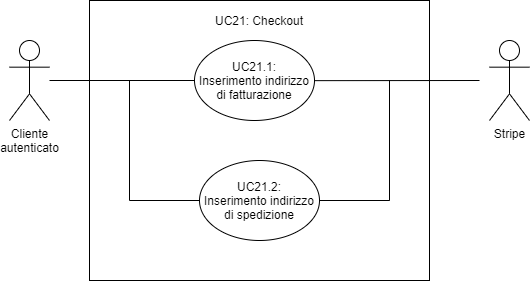
\includegraphics[scale=0.5]{../../../Images/AnalisiRequisiti/UC21}
    \centering
\end{figure}
\begin{itemize}
    \item \textbf{Descrizione:} caso d'uso per la creazione di un nuovo ordine e l'acquisto dei prodotti;
    \item \textbf{Attore Primario:} cliente autenticato;
    \item \textbf{Attore Secondario:} Stripe\textsubscript{\textbf{G}}, gestore di pagamenti di terze parti;
    \item \textbf{Precondizione:} il cliente si trova nel carrello (\hyperref[sec:UC11]{\underline{UC11}}) e ha già inserito almeno un prodotto oppure si trova nella pagina del prodotto (\hyperref[sec:UC4]{\underline{UC4}});
    \item \textbf{Input:} il cliente clicca il bottone per iniziare il checkout;
    \item \textbf{Postcondizione:} l'ordine viene emesso e aggiunto alla lista degli ordini di quel cliente; i prodotti acquistati vengono rimossi dal carrello e viene diminuita la rispettiva quantità dal deposito del venditore; il cliente viene reindirizzato alla pagina di riepilogo dell'ordine (\hyperref[sec:UC21]{\underline{UC21}})
    \item \textbf{Scenario Principale:}
          \begin{itemize}
              \item il cliente clicca il bottone per effettuare il checkout;
              \item il cliente inserisce i dati di fatturazione (\hyperref[sec:UC21.1]{\underline{UC21.1}}) e, se diversi, i dati di spedizione (\hyperref[sec:UC21.2]{\underline{UC21.2}});
              \item vengono inseriti eventuali costi di spedizione;
              \item il cliente viene reindirizzato al servizio di pagamento esterno, dove inserisce i dati di pagamento;
              \item l'ordine è emesso e segnato come completato.
          \end{itemize}
    \item \textbf{Estensioni:}
    \item Il cliente decide di non completare il checkout:
          \begin{itemize}
              \item  il cliente esce dalla pagina senza causare modifiche al carrello;
          \end{itemize}
    \item Il pagamento non è andato a buon fine
          \begin{itemize}
              \item L'utente ritorna al carrello \hyperref[sec:UC36]{\underline{UC36}}.
          \end{itemize}
\end{itemize}

\subsubsection{UC21.1: Inserimento dell'indirizzo di fatturazione}
\label{sec:UC21.1}
\begin{itemize}
    \item \textbf{Descrizione:} Sezione per l'inserimento dell'indirizzo fatturazione;
    \item \textbf{Attore Primario:} cliente autenticato;
    \item \textbf{Precondizione:} il cliente si trova nella fase di checkout;
    \item \textbf{Input:} il cliente inserisce i dati richiesti dalla pagina;
    \item \textbf{Postcondizione:} si procede con la fase successiva del checkout (\hyperref[sec:UC21.2]{\underline{UC21.2}})
    \item \textbf{Scenario Principale:} il cliente inserisce negli appositi spazi i dati per completare l'indirizzo di fatturazione.
\end{itemize}
\subsubsection{UC21.2: Inserimento dell'indirizzo di spedizione}
\label{sec:UC21.2}
\begin{itemize}
    \item \textbf{Descrizione:} Sezione per l'inserimento dell'indirizzo spedizione;
    \item \textbf{Attore Primario:} cliente autenticato;
    \item \textbf{Precondizione:} il cliente si trova nella fase di checkout;
    \item \textbf{Input:} il cliente inserisce i dati richiesti oppure clicca un apposito bottone se l'indirizzo di spedizione è lo stesso di quello di fatturazione;
    \item \textbf{Postcondizione:} si procede con la fase successiva del checkout;
    \item \textbf{Scenario Principale:} il cliente inserisce negli appositi spazi i dati per completare l'indirizzo di spedizione oppure clicca il pulsante per autocompletarli se è il medesimo di quello di fatturazione.
\end{itemize}
\subsubsection{UC21.3: Inserimento dei dati del pagamento}
\label{sec:UC21.3}
\begin{itemize}
    \item \textbf{Descrizione:} Sezione per l'inserimento dei dati di pagamento;
    \item \textbf{Attore Primario:} cliente autenticato;
    \item \textbf{Attore Secondario:} Stripe
    \item \textbf{Precondizione:} il cliente si trova nella piattaforma di Stripe per completare il checkout;
    \item \textbf{Input:} il cliente inserisce i dati richiesti dalla pagina;
    \item \textbf{Postcondizione:} il cliente ha inserito i dati per il pagamento;
    \item \textbf{Scenario Principale:} il cliente inserisce negli appositi spazi i dati della propria carta per il pagamento.
\end{itemize}
        \subsection{UC22: Annullamento checkout}
\label{sec:UC22}
\begin{itemize}
    \item \textbf{Descrizione:} visualizzazione di un errore per un fallimento nella fase di pagamento;
    \item \textbf{Attore Primario:} Stripe;
    \item \textbf{Precondizione:} il cliente ha inserito i dati del pagamento;
    \item \textbf{Input:} Stripe ritorna un errore nel risultato del pagamento;
    \item \textbf{Postcondizione:} viene visualizzato un messaggio di errore, successivamente il cliente viene reindirizzato alla sezione del checkout.
\end{itemize}

        \subsection{UC23: Visualizzazione della lista dei clienti}
\label{sec:UC23}
\begin{itemize}
    \item \textbf{Descrizione:} sezione per visualizzare l'elenco dei clienti del proprio negozio;
    \item \textbf{Attore Primario:} venditore autenticato; 
    \item \textbf{Precondizione:} il venditore si trova in una qualsiasi pagina;
    \item \textbf{Input:} il venditore clicca il bottone per entrare in questa sezione; 
    \item \textbf{Postcondizione:} il venditore visualizza la lista di tutti i clienti del negozio.
\end{itemize}
        \subsection{UC23: Visualizzazione della lista dei clienti}
\label{sec:UC23}
\begin{itemize}
    \item \textbf{Descrizione:} sezione per visualizzare l'elenco dei clienti del proprio negozio;
    \item \textbf{Attore Primario:} venditore autenticato; 
    \item \textbf{Precondizione:} il venditore si trova in una qualsiasi pagina;
    \item \textbf{Input:} il venditore clicca il bottone per entrare in questa sezione; 
    \item \textbf{Postcondizione:} il venditore visualizza la lista di tutti i clienti del negozio.
\end{itemize}
        \subsection{UC25: Visualizzazione della lista degli ordini}
\label{sec:UC25}
\begin{itemize}
    \item \textbf{Descrizione:} sezione per visualizzare l'elenco degli ordini effettuati dai clienti;
    \item \textbf{Attore Primario:} venditore autenticato; 
    \item \textbf{Precondizione:} il venditore si trova in una qualsiasi pagina della piattaforma;
    \item \textbf{Input:} il venditore clicca il bottone per entrare in questa sezione; 
    \item \textbf{Postcondizione:} il venditore visualizza la lista di tutti gli ordini effettuati dai suoi clienti.
\end{itemize}

        \subsubsection{UC26: Gestione delle categorie (\textbf{Aggiungere info specifiche})}
\label{sec:UC26}
\begin{figure}[!ht]
    \caption{Diagramma di UC26: Gestione delle categorie}
    \vspace{10px}
    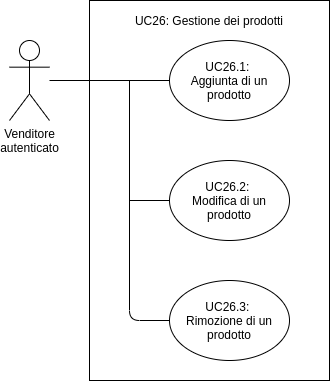
\includegraphics[scale=0.5]{../../../Images/AnalisiRequisiti/UC26}
    \centering
\end{figure}
\begin{itemize}
    \item \textbf{Descrizione:} sezione dove il venditore può gestire le categorie di prodotti del negozio;
    \item \textbf{Attore Primario:} venditore autenticato;
    \item \textbf{Precondizione:} il venditore si trova in una qualsiasi pagina della piattaforma;
    \item \textbf{Input:} il venditore clicca il bottone per entrare in questa sezione;
    \item \textbf{Postcondizione:} il venditore ha completato le operazioni sulle categorie;
    \item \textbf{Scenario Principale:}
          \begin{itemize}
              \item il venditore si trova nella pagina per la gestione del negozio;
              \item può decidere se aggiungere una nuova categoria o se rimuoverne una già presente;
              \item una volta terminato applica le modifiche.
          \end{itemize}
\end{itemize}
\subsubsubsection{UC26.1: Aggiunta di una categoria}
\label{sec:UC26.1}
\begin{itemize}
    \item \textbf{Descrizione:} sezione per aggiungere una categoria di prodotti nel negozio;
    \item \textbf{Attore Primario:} venditore autenticato;
    \item \textbf{Precondizione:} il venditore si trova nella sezione per gestire le categorie (\hyperref[sec:UC26]{\underline{UC26}});
    \item \textbf{Input:} il venditore inserisce tutti i dati relativi alla categoria da inserire;
    \item \textbf{Postcondizione:} la categoria è aggiunta e i clienti possono trovarla nel negozio;
    \item \textbf{Scenario Principale:}
          \begin{itemize}
              \item il venditore si trova nella sezione per gestire le categorie;
              \item il venditore decide di aggiungere una nuova categoria ed entra in questa sezione;
              \item inserisce tutti i dati richiesti;
              \item conferma l'aggiunta e la categoria è visibile nel negozio.
          \end{itemize}
\end{itemize}
\subsubsubsection{UC26.2: Rimozione di una categoria}
\label{sec:UC26.2}
\begin{itemize}
    \item \textbf{Descrizione:} sezione per rimuovere una categoria dal negozio;
    \item \textbf{Attore Primario:} venditore autenticato;
    \item \textbf{Precondizione:} il venditore si trova nella sezione per gestire le categorie (\hyperref[sec:UC26]{\underline{UC26}});
    \item \textbf{Input:} il venditore sceglie la categoria da rimuovere;
    \item \textbf{Postcondizione:} la categoria è stata rimossa dal negozio;
    \item \textbf{Scenario Principale:}
          \begin{itemize}
              \item il venditore si trova nella sezione per gestire le categorie;
              \item il venditore decide di rimuovere una categoria dal negozio;
              \item il venditore conferma la rimozione della categoria selezionata;
              \item la categoria non è più visibile nel negozio.
          \end{itemize}
\end{itemize}


        \subsubsection{UC27: Gestione delle categorie}
\label{sec:UC27}
\begin{figure}[!ht]
    \caption{Diagramma di UC27: Gestione delle categorie}
    \vspace{10px}
    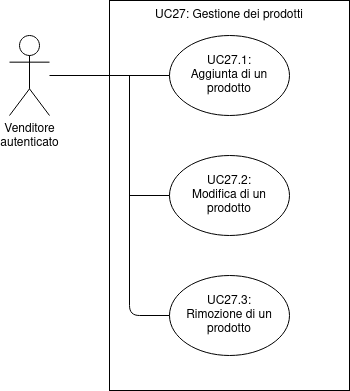
\includegraphics[scale=0.5]{../../../Images/AnalisiRequisiti/UC27}
    \centering
\end{figure}
\begin{itemize}
    \item \textbf{Descrizione:} sezione per il venditore, dove può gestire le categorie del negozio;
    \item \textbf{Attore Primario:} venditore autenticato;
    \item \textbf{Precondizione:} il venditore si trova in una qualsiasi pagina della piattaforma;
    \item \textbf{Input:} il venditore preme il bottone per entrare in questa sezione;
    \item \textbf{Postcondizione:} il venditore ha completato le operazioni sulle categorie;
    \item \textbf{Scenario Principale:}
          \begin{itemize}
              \item il venditore si trova nella pagina per la gestione del negozio;
              \item può decidere se aggiungere una nuova categoria o se rimuoverne una già presente;
              \item una volta terminato applica le modifiche.
          \end{itemize}
\end{itemize}
\subsubsubsection{UC27.1: Aggiunta di una categoria}
\label{sec:UC27.1}
\begin{itemize}
    \item \textbf{Descrizione:} sezione per aggiungere una categoria di prodotti nel negozio;
    \item \textbf{Attore Primario:} venditore autenticato;
    \item \textbf{Precondizione:} il venditore si trova nella sezione per gestire le categorie (\hyperref[sec:UC27]{\underline{UC27}});
    \item \textbf{Input:} il venditore inserisce tutti i dati relativi alla categoria da inserire;
    \item \textbf{Postcondizione:} la categoria è aggiunta e i clienti possono trovarlo nel negozio;
    \item \textbf{Scenario Principale:}
          \begin{itemize}
              \item il venditore si trova nella sezione per gestire le categorie;
              \item il venditore decide di aggiungere una nuova categoria ed entra in questa sezione;
              \item inserisce tutti i dati richiesti;
              \item conferma l'aggiunta e la categoria è visibile nel negozio.
          \end{itemize}
\end{itemize}
\subsubsubsection{UC27.2: Rimozione di una categoria}
\label{sec:UC27.2}
\begin{itemize}
    \item \textbf{Descrizione:} sezione per rimuovere una categoria dal negozio;
    \item \textbf{Attore Primario:} venditore autenticato;
    \item \textbf{Precondizione:} il venditore si trova nella sezione per gestire le categorie (\hyperref[sec:UC27]{\underline{UC27}});
    \item \textbf{Input:} il venditore sceglie la categoria da eliminare;
    \item \textbf{Postcondizione:} la categoria è stata rimossa dal negozio;
    \item \textbf{Scenario Principale:}
          \begin{itemize}
              \item il venditore si trova nella sezione per gestire le categorie;
              \item il venditore decide di rimuovere una categoria dal negozio;
              \item conferma;
              \item la categoria non è più visibile nel negozio.
          \end{itemize}
\end{itemize}


        \subsection{UC28: Aggiunta di un prodotto}
\label{sec:UC28}
\begin{itemize}
    \item \textbf{Descrizione:} sezione per aggiungere un prodotto nel negozio;
    \item \textbf{Attore Primario:} venditore autenticato;
    \item \textbf{Precondizione:} il venditore si trova nella sezione per gestire i prodotti;
    \item \textbf{Input:} il venditore inserisce tutti i dati relativi al prodotto da inserire;
    \item \textbf{Postcondizione:} il prodotto viene aggiunto e i clienti possono visualizzarlo nel negozio;
    \item \textbf{Scenario Principale:}
          \begin{itemize}
              \item il venditore si trova nella sezione per gestire i prodotti;
              \item il venditore decide di aggiungere un nuovo prodotto ed entra in questa sezione;
              \item il venditore inserisce tutti i dati richiesti:
                    \begin{itemize}
                        \item il nome del prodotto;
                        \item il prezzo di vendita esentasse;
                        \item la descrizione del prodotto;
                        \item la quantità disponibile in magazzino;
                        \item l'immagine che lo descrive;
                        \item la categoria del prodotto;
                        \item l'eventuale sconto.
                    \end{itemize}
              \item il venditore conferma l'aggiunta e il prodotto diviene disponibile nel negozio.
          \end{itemize}
\end{itemize}    